\documentclass[11pt,letterpaper]{article}
\usepackage[margin=1in]{geometry}
\usepackage[T1]{fontenc}
\usepackage{lmodern}
\usepackage{amsmath,amssymb,booktabs,array}
\usepackage{graphicx}
\usepackage[section]{placeins}
\usepackage[font=small,labelfont=bf]{caption}
\usepackage[numbers,sort&compress]{natbib}
\usepackage{xcolor}
\usepackage[colorlinks=true,allcolors=blue]{hyperref}
\usepackage{microtype}
\graphicspath{{figures/}}
% Generated by paper/gd-route/scripts/build_numbers.py from saved evidence; do not edit by hand.
% Each macro's source, SHA-256 and computation are listed in data/numbers.json.
\newcommand{\nUpdates}{20{,}000}
\newcommand{\nTail}{384}
\newcommand{\nMaxPeriod}{64}
\newcommand{\nChaosThreshold}{0.005}
\newcommand{\nMaps}{10}
\newcommand{\nCellsPerMap}{65{,}536}
\newcommand{\nProducerQualifying}{62}
\newcommand{\nAuditQualifying}{63}
\newcommand{\nConfirmed}{61}
\newcommand{\nCertificates}{154}
\newcommand{\nCertificatesVerified}{154}
\newcommand{\nPeriodMin}{4}
\newcommand{\nPeriodMax}{58}
\newcommand{\nOddWindows}{5}
\newcommand{\tOddPeriods}{5, 11, 13, 17 and 29}
\newcommand{\nConfirmedSOneR}{33}
\newcommand{\nConfirmedSTwo}{28}
\newcommand{\nRingReruns}{2{,}801}
\newcommand{\nChaosRerun}{160}
\newcommand{\nChaosKept}{157}
\newcommand{\pNotFixedMin}{87.1\%}
\newcommand{\pNotFixedMax}{99.97\%}
\newcommand{\nSOnePeriodic}{0}
\newcommand{\nNSSlices}{40}
\newcommand{\nNSCrossings}{35}
\newcommand{\nNSNotPeriodTwoStart}{5}
\newcommand{\xBirthMin}{0.1670}
\newcommand{\xBirthMax}{0.2401}
\newcommand{\xNSLowest}{1.650}
\newcommand{\tNSRoots}{2/11, 1/5, 2/9 and 3/13}
\newcommand{\xBirthAtSlice}{0.2180}
\newcommand{\xNSAtSlice}{1.738}
\newcommand{\xOnsetAtSlice}{1.738}
\newcommand{\xRhoOnset}{0.2180}
\newcommand{\tPlateausSTwo}{5/23, 7/32, 2/9 and 1/4}
\newcommand{\nFareySTwo}{3}
\newcommand{\nFareyPairsSTwo}{3}
\newcommand{\pFareyNullSTwo}{49\%}
\newcommand{\xTwoNinthsStart}{1.833}
\newcommand{\xTwoNinthsEnd}{1.879}
\newcommand{\tPlateausSOneR}{1/9, 2/17, 1/8, 3/23 and 2/15}
\newcommand{\nFareySOneR}{4}
\newcommand{\nFareyPairsSOneR}{4}
\newcommand{\pFareyNullSOneR}{100\%}
\newcommand{\nRaysFold}{1{,}316}
\newcommand{\nRaysFlip}{1{,}012}
\newcommand{\nRaysNS}{1{,}395}
\newcommand{\nRaysOther}{181}
\newcommand{\nRaysTotal}{3{,}904}
\newcommand{\nWindowsFoldFlip}{15}
\newcommand{\nWindowsNS}{41}
\newcommand{\nDraftShrimp}{2}
\newcommand{\nWFold}{46}
\newcommand{\nWFlip}{15}
\newcommand{\nWNS}{3}
\newcommand{\nWEdgeAgree}{61}
\newcommand{\nWEdgeCompared}{64}
\newcommand{\nWFlipTwoP}{10}
\newcommand{\nWOAllPlane}{65}
\newcommand{\nWOAllPlaneOf}{115}
\newcommand{\xWOAllPlaneNull}{1.57}
\newcommand{\nWOConfPlane}{31}
\newcommand{\nWOConfPlaneOf}{61}
\newcommand{\xWOConfPlaneNull}{4.92}
\newcommand{\nWOConfRefined}{35}
\newcommand{\nWOConfRefinedOf}{56}
\newcommand{\xWOConfRefinedNull}{3.58}
\newcommand{\nWOAllRefined}{78}
\newcommand{\nWOAllRefinedOf}{115}
\newcommand{\xWOAllRefinedNull}{7.43}
\newcommand{\nWOOdd}{0}
\newcommand{\nWOOddOf}{5}
\newcommand{\xWOOddNull}{0.17}
\newcommand{\nDoubledTongue}{7}
\newcommand{\xCertNewton}{10^{-10}}
\newcommand{\xCertAtol}{10^{-9}}
\newcommand{\xCertRtol}{10^{-8}}
\newcommand{\xCertCandidate}{10^{-3}}
\newcommand{\xCertDivisor}{10^{-6}}
\newcommand{\xCertMargin}{10^{-7}}
\newcommand{\nCertIterations}{60}
\newcommand{\nMinComponent}{4}
\newcommand{\nGateMinPeriod}{3}
\newcommand{\pRingFraction}{50\%}
\newcommand{\xScreenAtol}{10^{-8}}
\newcommand{\xScreenRtol}{10^{-6}}
\newcommand{\nMinRepeats}{6}
\newcommand{\nFtleSteps}{4{,}000}
\newcommand{\nFtleAlign}{1{,}000}
\newcommand{\pDrift}{1\%}
\newcommand{\xDivergence}{10^{8}}
\newcommand{\nScoreHorizon}{1{,}000}
\newcommand{\nRingSteps}{30{,}000}
\newcommand{\nRingFtle}{10{,}000}
\newcommand{\nRingCap}{48}
\newcommand{\nChaosPerMap}{16}
\newcommand{\nAuditChecked}{154}
\newcommand{\nAuditAllOk}{154}
\newcommand{\xAuditMaxRadiusDiff}{1.7\times10^{-7}}
\newcommand{\nAuditReceiptFiles}{276}
\newcommand{\nAuditMismatched}{0}
\newcommand{\nCertPThree}{129}
\newcommand{\nConfTrivial}{4}
\newcommand{\nConfTrivialPass}{4}
\newcommand{\nConfRefinedExcluded}{5}
\newcommand{\tConfRefinedExcluded}{4, 4, 6, 6 and 8}
\newcommand{\nLevelZeroPass}{28}
\newcommand{\tShiftCounts}{$m=1$ for 19, $m=2$ for 8 and $m=3$ for 1}
\newcommand{\xRhoMinSlice}{0.2158}
\newcommand{\xRhoMinAt}{1.780}
\newcommand{\nBetweenCells}{168}
\newcommand{\nBetweenChaotic}{167}
\newcommand{\xQuarterStart}{1.909}
\newcommand{\xQuarterEnd}{1.919}
\newcommand{\xFigSixQPRho}{0.2159}
\newcommand{\xFigSixQPFtle}{0.0001}
\newcommand{\xFigSixLockRho}{0.2222}
\newcommand{\xFigSixLockFtle}{-0.0072}
\newcommand{\xFigSixChaosRho}{0.2298}
\newcommand{\xFigSixChaosFtle}{0.0504}


\definecolor{placeholderframe}{HTML}{EB6834}
\definecolor{placeholderfill}{HTML}{FDF0EA}
\definecolor{noticefill}{HTML}{F0EFEC}
\newcommand{\placeholder}[1]{\par\medskip\noindent\fcolorbox{placeholderframe}{placeholderfill}{%
  \parbox{\dimexpr\linewidth-2\fboxsep-2\fboxrule\relax}{\small\textbf{Placeholder.} #1}}\par\medskip}
\newcommand{\notice}[1]{\par\medskip\noindent\fcolorbox{gray}{noticefill}{%
  \parbox{\dimexpr\linewidth-2\fboxsep-2\fboxrule\relax}{\small #1}}\par\medskip}
\newcommand{\confirmedlabel}{\textsc{confirmed (prospectively designed, independently audited)}}
\newcommand{\exploratorylabel}{\textsc{exploratory}}
\newcommand{\provenance}[2]{\textit{Generated by} \texttt{#1}; \textit{receipt} \texttt{#2}.}

\hypersetup{pdftitle={Beyond the edge of stability: periodic windows, quasi-periodicity and phase locking in the learning-rate plane of gradient descent},
  pdfsubject={Private working draft}}

\title{Beyond the edge of stability: periodic windows, quasi-periodicity\\
and phase locking in the learning-rate plane of gradient descent}
\author{Authorship to be finalized by the human researcher}
\date{Private working draft, not for distribution}

\begin{document}
\maketitle

\notice{\textbf{AI-use disclosure.} Generative-AI tools helped implement, audit, execute, interpret, visualize,
review, and draft this study. The author selected the research question, authorized the compute, has inspected
the artifacts, and is responsible for the final text and claims. This is an independent, non-peer-reviewed
preprint. Verify numbers against the released receipts before relying on them.\\[2pt]
\textit{Draft note: every clause above must be confirmed by the author before release.}}

\begin{abstract}
Full-batch gradient descent with a large learning rate can oscillate, cycle or behave chaotically instead of
settling. Trainability maps over learning-rate planes record a binary convergent-or-divergent label, which
conflates these dynamical regimes. We resolve the dynamics behind such maps in two small tanh networks trained
with separate learning rates for their two layers, and we organize the results around one thesis: beyond the edge
of stability, the period-2 oscillation gives way to quasi-periodic training and phase-locked periodic windows.

(1) Confirmed in a prospectively designed and independently audited study: the learning-rate planes contain
\nConfirmed{} numerically certified attracting periodic orbits of the full parameter-space update map, with
periods from \nPeriodMin{} to \nPeriodMax{}, whose domains are surrounded mainly by rerun-confirmed chaos. In six
coarse maps, \pNotFixedMin{} to \pNotFixedMax{} of the cells that a published binary convergence score labels
convergent were not classified as fixed points after \nUpdates{} updates.

(2) Exploratory: on all \nNSCrossings{} traced slices that start on the edge-of-stability period-2 orbit, that
orbit loses stability as a complex pair of two-step multipliers crosses the unit circle, a Neimark--Sacker
candidate. On one slice the crossing angle is \xBirthAtSlice{} turns per two steps and the first quasi-periodic
cell rotates at \xRhoOnset{}. Of \nWOConfRefinedOf{} eligible windows, \nWOConfRefined{} pass a Birkhoff ordering
test of their projected orbits, against at most \xWOConfRefinedNull{} expected by chance. Only \nDraftShrimp{} of
\nConfirmed{} windows meet draft criteria for classical shrimp anatomy.

Takeaway: the region that a binary map calls trainable holds certified periodic windows inside chaos, and
exploratory evidence ties them to quasi-periodic training born where the period-2 orbit acquires complex
multipliers. The claim we test next is local: a period-2 branch undergoes an attracting Neimark--Sacker
bifurcation and a rule-selected window is connected to its resonance by continuation. Nothing here concerns
stochastic or large-scale training or establishes a training benefit.
\end{abstract}

\noindent\textbf{Study status.} Results labeled \confirmedlabel{} come from the map study of
Section~\ref{sec:confirmed}, whose design, thresholds and analysis were pushed before outcomes and repeated by an
independent audit. Results labeled \exploratorylabel{} (Section~\ref{sec:route}) were found while exploring and
have not been tested on held-out networks. Provenance for every figure and number is described in
Section~\ref{sec:repro}.

\section{Introduction}
\label{sec:intro}

Training with a learning rate beyond the classical stability limit is common practice. At the edge of stability,
the sharpness of the loss hovers near $2/\eta$ while the loss still decreases over long horizons
\citep{cohen2021}; self-stabilization explains how sharpness is held there \citep{damian2023}, progressive
sharpening how it gets there \citep{agarwala2023}, and the catapult phase what happens to the loss at somewhat
larger rates \citep{lewkowycz2020}. Simplified models show period doubling and chaos as the step size grows
\citep{kalra2025,chen2024phases,hofmann2026}. Over two-dimensional hyperparameter planes, the boundary between
trainable and divergent settings is fractal \citep{sohldickstein2024,torkamandi2025,liu2024,liang2026}. These maps
record whether the loss falls and stays bounded, not what the parameters do.

We ask what the dynamics inside such maps are. We treat full-batch gradient descent with separate learning rates
for the hidden and output layers as a two-parameter family of maps on parameter space. For every cell of a
learning-rate grid we screen the parameter state at the end of a long run (fixed point, periodic orbit with its
period, chaos, drift, divergence), certify selected periodic orbits with Newton's method on the exact Jacobian,
and follow orbits and their stability boundaries through the plane.

\paragraph{Thesis and status.} We organize the results around one thesis: beyond the edge of stability, the
period-2 oscillation gives way to quasi-periodic training on an invariant circle, rational rotation numbers lock
into periodic windows, and the windows of the learning-rate plane are largely these locked orbits. Each result
below says exactly what passed. The certified windows and the comparison with the binary score are confirmed.
The complex-pair crossings, rotation numbers, ordering tests and staircases are exploratory; we call the crossings
Neimark--Sacker candidates until transversality, nondegeneracy and an attracting invariant circle are documented.
The claim we will test on held-out networks is local and existential: in specified finite tanh networks under
deterministic full-batch gradient descent in float64, a period-2 branch undergoes an attracting Neimark--Sacker
bifurcation and a rule-selected window is connected to the corresponding resonance by continuation.

\paragraph{Prior work.} Periodic windows, period doubling, positive Lyapunov exponents and broadband power
spectra in learning dynamics, with the learning rate as bifurcation parameter, date back at least to
\citet{vandermaas1990}, who studied a three-unit autoassociator. Their delay-embedded chaotic attractors are thin
folded curves, effectively one-dimensional chaos of the period-doubling kind, unlike the invariant circles of the
two-step map studied here. Period-colored maps over optimizer
hyperparameters have been drawn from a two-dimensional projection of the error, without full-state verification
\citep{sveleba2026}. \citet{hofmann2026} studies finite-step gradient descent as a dynamical system in solvable
models: the edge of stability as the first (flip) bifurcation of the training map, the period-doubling route with
windows, and, in a two-mode depth-two linear network, a ``rotational edge'' beyond which the unstable multipliers
of the aligned 2-cycle are complex and the system saturates in a persistently misaligned oscillatory state. Our
analysis starts where that result stops: we ask whether such a crossing produces quasi-periodic training whose
rotation is set by the crossing multiplier, and whether periodic windows are its resonances. Riddled basins and
learning-rate-dependent reproducibility are documented by \citet{ly2025}. Invariant curves and phase-locking Arnold
tongues appear in a multiplicative-weights learning rule for population games \citep{metaxas2026}, and chaos in
learning a two-person game goes back to \citet{sato2002}; both concern games rather than descent on one loss.
Heavy-ball momentum has cycles that rotate by $1/K$ \citep{goujaud2025}.

\paragraph{This paper's contribution.}
\begin{itemize}
\item Confirmed: a period-resolved description of the learning-rate plane of full-batch gradient descent in two
small networks, with \nConfirmed{} certified attracting windows embedded in chaos, repeated by an independent audit.
\item Confirmed: a cell-by-cell comparison with the published binary convergence score, which conflates
fixed points, periodic orbits, chaos and drift.
\item Exploratory: complex-pair crossings of the period-2 orbit along a traced curve, rotation numbers of the
quasi-periodic training that follows, a Birkhoff ordering test of the windows against a null, and rotation-number
staircases.
\item Code, receipts and a verification script that re-derive every figure and number.
\end{itemize}

\paragraph{Not claimed.}
\begin{itemize}
\item No Neimark--Sacker bifurcation in the strict sense: transversality, nondegeneracy and an attracting
invariant circle are not yet documented.
\item No route to chaos: no prespecified connected path through sustained chaos has been tested.
\item No proof that the windows are Arnold tongues: the Birkhoff test is a diagnostic of projected orbits, and
resonance ancestry is pending.
\item No claim about stochastic, minibatch or large-scale training, other architectures or real data, and no
training benefit.
\end{itemize}

\section{Gradient descent as a family of maps}
\label{sec:background}

Let $L(\theta)$ be the full-batch training loss of a network with parameters $\theta\in\mathbb{R}^n$, split
into hidden-layer and output-layer blocks. Gradient descent with per-layer learning rates is the map
\begin{equation}
\theta_{t+1} = F(\theta_t) = \theta_t - P\,\nabla L(\theta_t), \qquad
P = \operatorname{diag}(\eta_h \mathbf{1}_{\text{hidden}}, \eta_o \mathbf{1}_{\text{output}}),
\label{eq:map}
\end{equation}
a family of maps indexed by the two rates $(\eta_h,\eta_o)$. Its Jacobian is $DF(\theta) = I - P H(\theta)$
with $H$ the Hessian of $L$. An orbit of period $p$ is stable when all eigenvalues (multipliers) of
$DF(\theta_{p-1})\cdots DF(\theta_0)$ lie inside the unit circle. Generically it loses stability when a
multiplier crosses the circle: at $+1$ (fold), at $-1$ (flip, which doubles the period) or as a complex pair
$e^{\pm 2\pi i\omega}$ (Neimark--Sacker, which under transversality and nondegeneracy conditions creates an
invariant closed curve) \citep{kuznetsov2019}.

\paragraph{Why the candidates start at period 2.} $DF(\theta)$ is similar to the symmetric matrix
$I - P^{1/2} H P^{1/2}$, so at a fixed point all multipliers are real and a fixed point loses stability by fold or
flip only. The edge-of-stability oscillation is the period-2 orbit born at that flip. For a period-2 orbit
$\{\theta_a,\theta_b\}$, the two-step Jacobian is similar to $S_b S_a$ with
$S_j = I - P^{1/2} H(\theta_j) P^{1/2}$. A product of two symmetric matrices has real eigenvalues when one factor
is positive definite, but at the edge of stability each $S_j$ has a negative eigenvalue in the oscillating
direction, so complex multipliers become possible. This is an elementary observation; complex unstable
multipliers of an edge-of-stability 2-cycle were derived for a two-mode linear network by \citet{hofmann2026}.

\paragraph{Circle maps and phase locking.} On an invariant circle the dynamics has a rotation number $\rho$, the
mean fraction of a turn per iterate. When $\rho = m/q$ is rational the motion can lock onto a periodic orbit; the
locked parameter sets are Arnold tongues, rotation numbers along a parameter path form a devil's staircase, and
the widest plateau between two locked rationals is typically their Farey mediant
\citep{arnold1965,jensen1983,jensen1984}. Breakdown of the circle leads to chaos
\citep{curry1978,aronson1982,ostlund1983}. Because the circle in question belongs to the two-step map, a locked
orbit at rotation $m/q$ has period $2q$ for $F$; this relation is a consequence of the setting, not evidence.

\paragraph{Shrimps.} In two-parameter families of dissipative maps, periodic windows inside chaos often take a
characteristic ``shrimp'' shape bounded by fold and flip curves \citep{gallas1993,gallas1994}. We test for this
anatomy explicitly rather than assume it.

\section{Methods}
\label{sec:methods}

% Generated by paper/gd-route/scripts/build_numbers.py from the frozen plan and summary; do not edit.
\begin{table}[htbp]
\centering\small
\setlength{\tabcolsep}{3.5pt}
\begin{tabular}{@{}l r >{\raggedright\arraybackslash}p{2.6cm} >{\raggedright\arraybackslash}p{3.6cm} l >{\raggedright\arraybackslash}p{1.4cm} >{\raggedright\arraybackslash}p{1.7cm}@{}}
\toprule
Network & Parameters & Training points & Architecture & Weight decay & Seeds & Maps \\
\midrule
S1 & 72 & 72 standard-normal & 8 inputs, 8 tanh units, no biases, mean-field & 0 & 28001, 28002 & 2 coarse \\
S1R & 72 & 72 standard-normal & 8 inputs, 8 tanh units, no biases, mean-field & $10^{-3}$ & 28001, 28002 & 2 coarse, 2 zoom \\
S2 & 13 & 24 from a tanh teacher & 2 inputs, 3 tanh units, biases & $10^{-3}$ & 28011, 28012 & 2 coarse, 2 zoom \\
\bottomrule
\end{tabular}
\caption{\textbf{Design of the map study.} Every map has $256\times256$ logarithmically spaced pairs of hidden- and output-layer rates; coarse maps span 3 decades in each rate and zoom maps 0.36 decades. Every cell runs 20{,}000 full-batch updates in float64 from its seed's initial parameters. S1 is the published configuration of the fractal-trainability study and is reported descriptively.}
\label{tab:design}
\end{table}


\paragraph{Networks and data.} Table~\ref{tab:design} lists the design. S1 reproduces the published mean-field
configuration of the fractal-trainability study \citep{sohldickstein2024}; S1R adds weight decay; S2 is a
13-parameter tanh regressor fitted to points from a random tanh teacher. We refer to a network and seed together,
for example S2-28011. Training is deterministic full-batch gradient descent in float64.

\paragraph{Three different quantities.} The published binary score measures loss reduction: a run counts as
convergent when its loss, normalized by the initial loss and averaged over the last 20 of the first
\nScoreHorizon{} updates, is below one \citep{sohldickstein2024}. Our screening labels classify the parameter state
at the end of a finite run. Certification validates individual periodic orbits. The three need not agree, and we
compare them cell by cell.

\paragraph{Screening.} Every cell runs \nUpdates{} updates from the seed's initial parameters. The last \nTail{}
updates are screened for the smallest full-state recurrence period up to \nMaxPeriod{}: a period $p$ requires the
state to recur with componentwise tolerance $\xScreenAtol + \xScreenRtol\,|\theta|$ over the whole tail, which
spans at least \nMinRepeats{} repeats. The largest finite-time Lyapunov exponent (FTLE) is averaged over the last
\nFtleSteps{} updates after \nFtleAlign{} updates of tangent alignment. Labels are fixed point, periodic, chaotic
(FTLE above \nChaosThreshold{} per update), drift (parameter norm still growing by more than \pDrift{} over the FTLE
window), unresolved, or divergent (non-finite or larger than $\xDivergence$).

\paragraph{Numerically certified.} An orbit of period $p$ is numerically certified when damped Newton iteration
on $F^p(\theta)-\theta=0$, using the exact chain-rule Jacobian of $F^p$, reaches an undamped relative correction
below $\xCertNewton$ within \nCertIterations{} iterations; the converged point closes to within
$\xCertAtol + \xCertRtol\,|\theta|$ in every component; it lies within $\xCertCandidate$ (relative) of the
screened candidate; every proper-divisor iterate is separated from it by at least $\xCertDivisor$ (relative), so
the period is primitive; and it is attracting when the spectral radius of the monodromy matrix is below
$1-\xCertMargin$. This is a floating-point verification, not a computer-assisted proof.

\paragraph{Embedded windows and audit.} A connected component of equal-period cells qualifies as an embedded
window when its period is at least \nGateMinPeriod{}, it has at least \nMinComponent{} cells, no cell of its
exterior ring is a fixed point or has a proper-divisor period, at least \pRingFraction{} of the ring is
rerun-confirmed chaos (reruns of \nRingSteps{} updates with a \nRingFtle{}-update FTLE and a different tangent
vector, up to \nRingCap{} ring cells per component), and its representative orbit is certified and attracting.
The audit was a separate program that imports neither the batched engine, the orbit certifier nor the selection
helpers: it rewrote the one-cell map, the recurrence screen, the zoom rule and the component and ring rules,
rechecked every certificate with finite-difference Jacobians (all \nAuditAllOk{} of \nAuditChecked{} pass closure,
primitivity, stability and seed checks; spectral radii agree within $\xAuditMaxRadiusDiff$), re-simulated the
ring cells of every qualifying component, recomputed the gate on its own evidence, and found \nAuditMismatched{}
mismatches among the \nAuditReceiptFiles{} receipt files.

\paragraph{Continuation and boundary type.} From the center of a window, its certified orbit is continued along
64 rays in the rate plane until it loses stability, located by bisection, and the boundary is typed by the
crossing multiplier: fold ($+1$), flip ($-1$) or complex pair. We do not check transversality or nondegeneracy,
so all three types are candidates; we write ``Neimark--Sacker candidate'' for the complex-pair case because the
thesis rests on it. The same procedure traces where the period-2 orbit loses stability along slices of fixed
output rate.

\paragraph{Rotation numbers and the Birkhoff test.} For a non-periodic cell we take the two-step samples
$z_k=\theta_{2k}$, project them on their first two principal axes, and define the rotation number as the mean
unwrapped angle increment in turns per two steps. For a certified orbit of period $p$ we take its two-step points
($q=p/2$ points for even $p$, $q=p$ for odd $p$), sort them by angle in their principal plane, and say the orbit
passes when every step advances the angular rank by the same shift $m$ with $\gcd(m,q)=1$, the ordering of a
Birkhoff orbit of rotation $m/q$. The number of points $q$, and therefore the relation $p=2q$, is fixed by the
period; what the test measures is the ordering and the shift. Orbits with 2 or 3 points pass by construction. The
null is the pass probability of the same test for uniformly random angles; for a group of orbits we report the
expected number of chance passes. The refined test also orders points along the shortest closed tour through them
and tests the points of $F^{2^{k+1}}$ ($k=1,2,3$), which can detect orbits born by period doubling inside a
locked window; it counts only tests on at least 5 points, and its null for each orbit is the sum of the per-test
pass probabilities (a union bound), so the summed null is an upper bound on the expected number of chance passes.

\section{Periodic windows inside chaotic training}
\label{sec:confirmed}

\noindent Status: \confirmedlabel.

\begin{figure}[htbp]
\centering
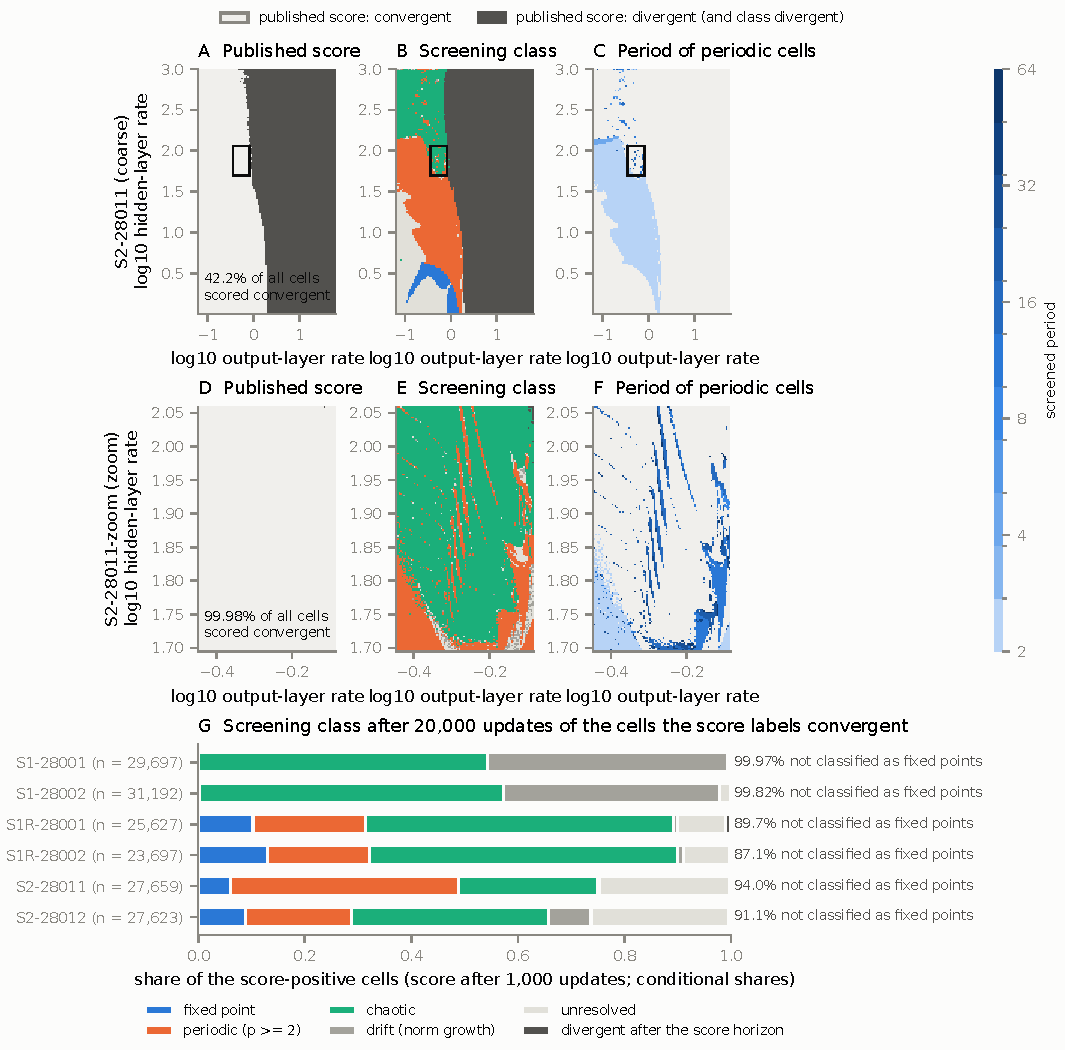
\includegraphics[width=\linewidth]{f1_binary_vs_period.pdf}
\caption{\textbf{The binary score conflates dynamical regimes: the cells it labels convergent carry fixed-point,
periodic, chaotic and drift labels after \nUpdates{} updates.} Panels A and D show the published score after
\nScoreHorizon{} updates; the printed share is the fraction of all cells in that map scored convergent. Panels B,
C, E and F show the screening class and, for periodic cells, the period of the same cells after \nUpdates{}
updates (S2-28011, coarse and zoomed; the rectangle marks the zoom). Panel G is conditional: among the cells the
score labels convergent, the share in each screening class, for all six coarse maps. Screening labels are
finite-time labels; only certified orbits are verified.
\provenance{paper/gd-route/figures/f1\_binary\_vs\_period.py}{figures/f1\_binary\_vs\_period.provenance.json}}
\label{fig:binary}
\end{figure}

The learning-rate planes of S1R and S2 contain \nConfirmed{} embedded windows that qualify on both the producer's
and the auditor's evidence (\nProducerQualifying{} and \nAuditQualifying{} respectively; the disagreements all sit
at the \pRingFraction{} ring threshold). All \nCertificates{} attempted orbit certifications verified. Confirmed
periods range from \nPeriodMin{} to \nPeriodMax{} and include the odd periods \tOddPeriods{}. The exterior rings
were checked with \nRingReruns{} reruns, and \nChaosKept{} of \nChaosRerun{} randomly chosen chaotic cells
(\nChaosPerMap{} per map) stayed chaotic on a rerun with a different tangent vector.

Figure~\ref{fig:binary} compares these dynamics with the published binary score. In the six coarse maps,
\pNotFixedMin{} to \pNotFixedMax{} of the cells the score labels convergent were not classified as fixed points
after \nUpdates{} updates; the score's success means the loss fell, not that the parameters settled. Task success
and non-convergent learning dynamics can coexist: \citet{vandermaas1990} reported that their network performed
its task across the whole learning-rate range they studied, including where learning was chaotic. The
published configuration without weight decay (S1) has \nSOnePeriodic{} periodic cells in both seeds: its runs
diverge, stay chaotic, or drift toward large weights while the loss slowly falls. Adding weight decay makes the
windows appear.

\section{Exploratory evidence for the thesis}
\label{sec:route}

\noindent Status: \exploratorylabel{}. The analyses in this section were chosen while exploring and used data
that shaped the thesis.

\subsection{The period-2 orbit acquires complex multipliers: Neimark--Sacker candidates}

\begin{figure}[htbp]
\centering
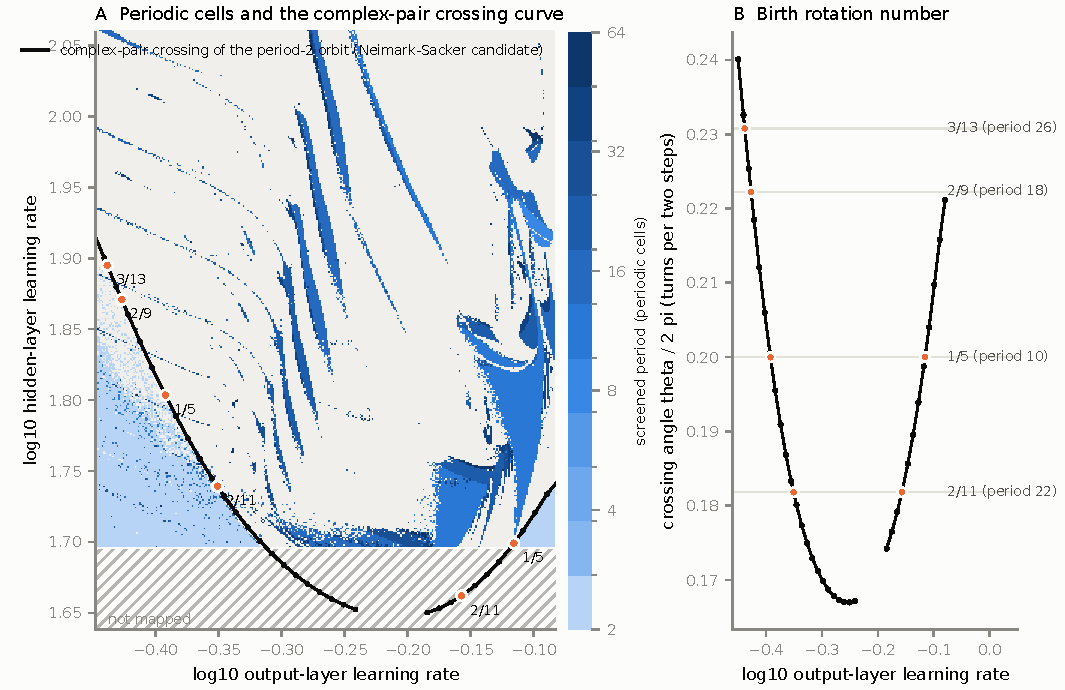
\includegraphics[width=\linewidth]{f2_ns_tongue_roots.pdf}
\caption{\textbf{Along the whole traced curve, the edge-of-stability period-2 orbit loses stability as a complex
pair of two-step multipliers crosses the unit circle (Neimark--Sacker candidates).} A: periodic cells of a
$1{,}024\times1{,}024$ map (shade: period), the traced crossing curve (black) and the resonance points where the
crossing angle equals a rational $m/q$ with $q\le 13$ (orange); tongues would be rooted there if the crossings are
nondegenerate Neimark--Sacker bifurcations. B: crossing angle along the curve. On \nNSNotPeriodTwoStart{} of
\nNSSlices{} slices the starting point was not on the period-2 orbit; those slices break the curve. Resonance
points are interpolated between traced slices, and tongues near their roots are narrower than one map cell.
\provenance{paper/gd-route/figures/f2\_ns\_tongue\_roots.py}{figures/f2\_ns\_tongue\_roots.provenance.json}}
\label{fig:ns}
\end{figure}

We continued the period-2 orbit of S2-28011 toward larger hidden-layer rates along \nNSSlices{} slices of fixed
output rate. On all \nNSCrossings{} slices that started on it, the orbit loses stability as a complex pair of
two-step multipliers crosses the unit circle (Figure~\ref{fig:ns}). The crossing curve is U-shaped, with its
lowest point at $\log_{10}\eta_h = \xNSLowest{}$, and the crossing angle $\omega$ ranges from \xBirthMin{} to
\xBirthMax{} turns per two steps, passing the resonances \tNSRoots{}.

On the slice through the period-18 window, the curve interpolated to that slice places the crossing at
$\log_{10}\eta_h = \xNSAtSlice{}$ with $\omega = \xBirthAtSlice{}$; in an independent staircase computation the
first quasi-periodic cell lies at \xOnsetAtSlice{} and rotates at \xRhoOnset{}. Agreement of the rotation number
with the crossing angle is what a Neimark--Sacker bifurcation predicts, but it does not establish one: the
transversality of the crossing, the nondegeneracy (first Lyapunov) coefficient and an attracting invariant circle
with converged residuals remain to be documented.

\placeholder{Rotation-number map of the S2-28011 plane overlaid with the crossing curve, testing whether the
rotation just beyond the curve equals the crossing angle everywhere along it (computation in progress).}

\placeholder{Resonance ancestry: continuation of a rule-selected window (the $1/5$ window) through both of its
fold edges back to the $1/5$ resonance on the crossing curve, with the onset, circle and detuning acceptance rules
frozen before any confirmation (in progress).}

\subsection{States along one slice}

\begin{figure}[htbp]
\centering
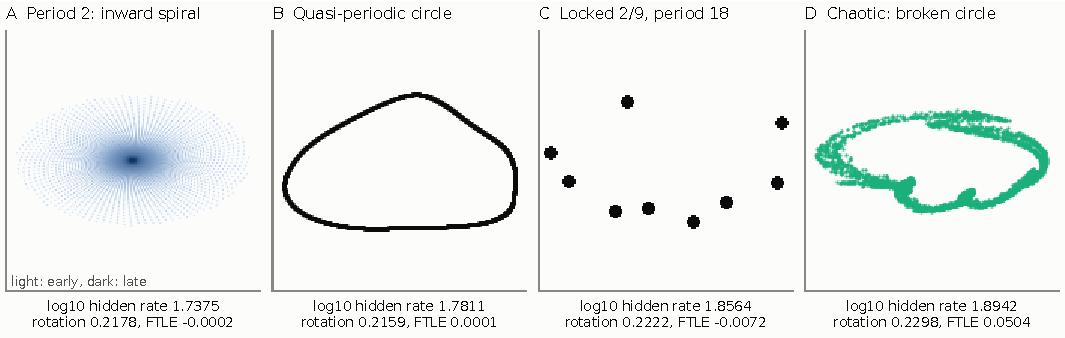
\includegraphics[width=\linewidth]{f6_route_portraits.pdf}
\caption{\textbf{Four states along one slice, in order of increasing hidden-layer rate: an inward spiral to the
2-cycle, a closed invariant curve, nine locked points and a broken curve.} Each panel shows every second parameter
vector of one run projected on its own two principal axes. The rates are chosen by a fixed rule from the staircase
receipt (the period-2 cell closest to the onset, the median quasi-periodic cell, the middle of the longest $2/9$
plateau, the median chaotic cell between the $2/9$ and $1/4$ plateaus), not by eye. The states are not a monotone
sequence: beyond the onset the rotation number first falls, and beyond panel D training locks again at $1/4$
before chaos returns (Figure~\ref{fig:staircase}). Projections onto two axes can hide structure in the remaining
dimensions.
\provenance{paper/gd-route/figures/f6\_route\_portraits.py}{figures/f6\_route\_portraits.provenance.json}}
\label{fig:portraits}
\end{figure}

Figure~\ref{fig:portraits} shows what training looks like along that slice. Beyond the crossing, the two-step
samples lie on a closed curve (rotation \xFigSixQPRho{}, FTLE \xFigSixQPFtle{}); inside the period-18 window they
are nine points (rotation \xFigSixLockRho{}, FTLE \xFigSixLockFtle{}); between the $2/9$ and $1/4$ plateaus the
curve thickens and breaks (FTLE \xFigSixChaosFtle{}).

\subsection{Rotation numbers form staircases}

\begin{figure}[htbp]
\centering
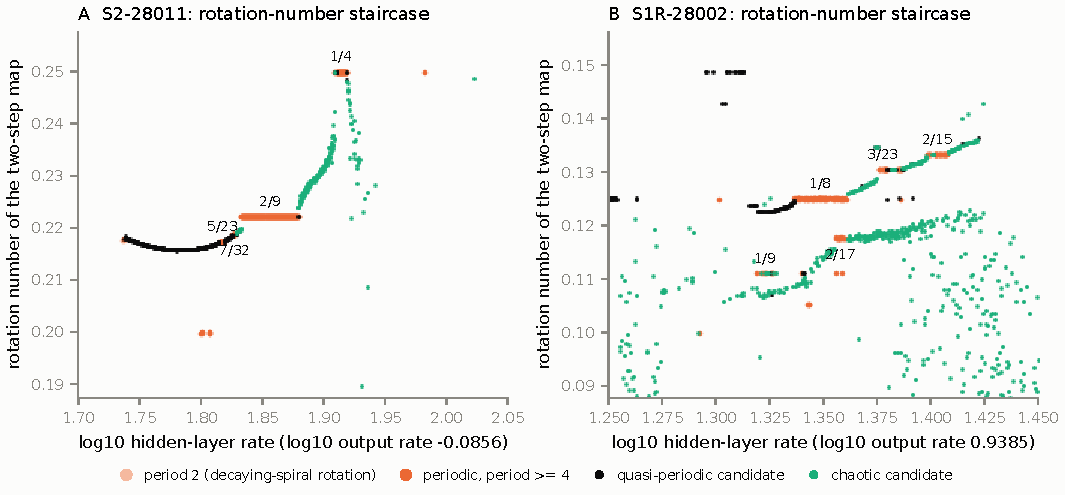
\includegraphics[width=\linewidth]{f3_staircases.pdf}
\caption{\textbf{Along slices, quasi-periodic cells trace continuous rotation numbers and periodic cells sit on
rational plateaus.} Plateaus are detected automatically (locked cells with period $2q$ or a doubling of it,
rotation within $6\times10^{-4}$ of $m/q$) and labeled when they hold at least 8 cells. In S2 the rotation number
first falls after the onset, then rises; the cells between the $2/9$ and $1/4$ plateaus are almost all chaotic
candidates. In S1R two rotation branches coexist over the same rates, a sign of coexisting attractors. Chaotic
cells outside the plotted range are not shown.
\provenance{paper/gd-route/figures/f3\_staircases.py}{figures/f3\_staircases.provenance.json}}
\label{fig:staircase}
\end{figure}

Along the slice through the period-18 window of S2-28011 (Figure~\ref{fig:staircase}), the rotation number falls
from \xRhoOnset{} at the onset to \xRhoMinSlice{} at $\log_{10}\eta_h = \xRhoMinAt{}$, then rises and locks at
$2/9$ for $\log_{10}\eta_h$ from \xTwoNinthsStart{} to \xTwoNinthsEnd{}. Of the \nBetweenCells{} cells between the
$2/9$ and $1/4$ plateaus, \nBetweenChaotic{} are chaotic candidates; training then locks at $1/4$ from
\xQuarterStart{} to \xQuarterEnd{} before chaos returns. The labeled plateaus are \tPlateausSTwo{} in S2 and
\tPlateausSOneR{} in S1R. Consecutive plateaus are Farey neighbors ($|m_1 q_2 - m_2 q_1| = 1$) in \nFareySTwo{} of
\nFareyPairsSTwo{} pairs in S2, against \pFareyNullSTwo{} per pair for randomly drawn fractions in the same range,
and in \nFareySOneR{} of \nFareyPairsSOneR{} pairs in S1R, where the null is \pFareyNullSOneR{} because every
fraction with a small enough denominator in that range appears. The Farey pattern is weak evidence in S2 and
uninformative in S1R.

\subsection{A Birkhoff ordering test of the windows}

\begin{figure}[htbp]
\centering
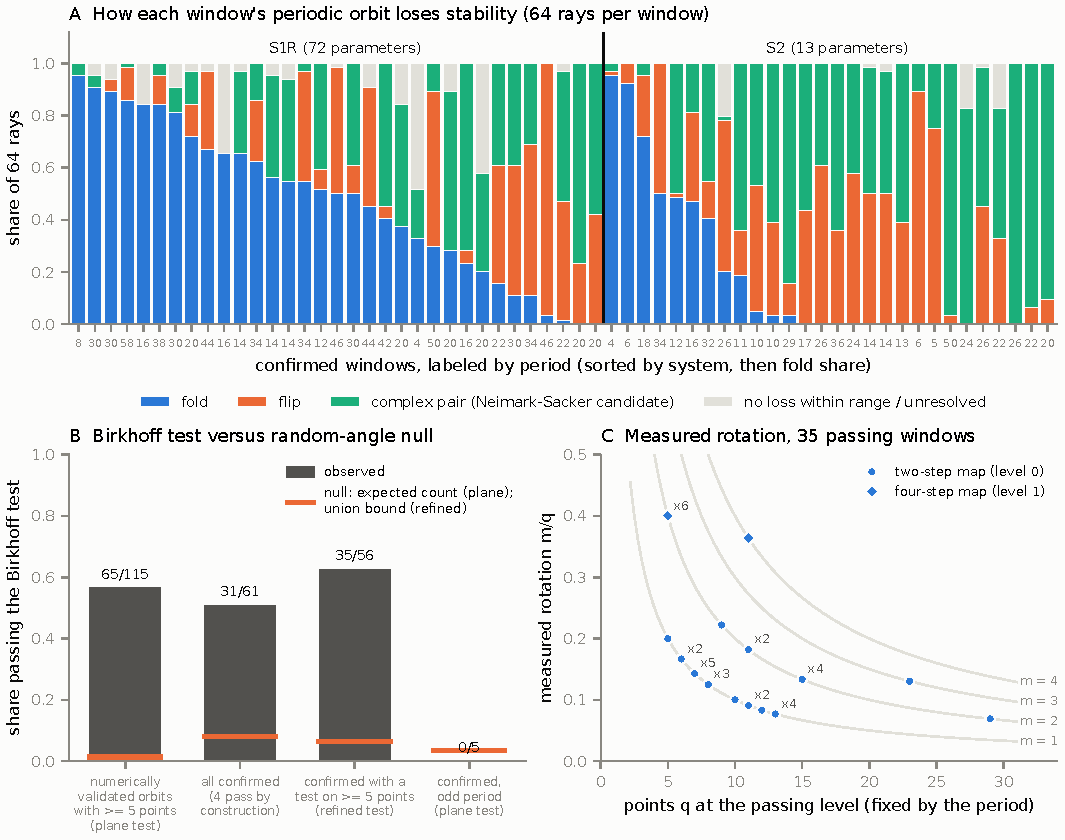
\includegraphics[width=\linewidth]{f5_window_census.pdf}
\caption{\textbf{Across all \nConfirmed{} windows, stability boundaries mix fold, flip and complex-pair crossings,
and most eligible windows pass a Birkhoff ordering test far above its null.} A: boundary type along 64 rays per
window. B: share of orbits passing the test (gray) against the null (orange): the expected share of chance passes
for the plane test, and the union bound for the refined test; eligibility is printed under each bar. C: rotation
$m/q$ measured by the passing test at its first passing level; $q$ is fixed by the period and level by
construction, so only the shift $m$ and the ordering are measured.
\provenance{paper/gd-route/figures/f5\_window\_census.py}{figures/f5\_window\_census.provenance.json}}
\label{fig:census}
\end{figure}

Across the \nConfirmed{} windows, the \nRaysTotal{} rays end at \nRaysFold{} folds, \nRaysFlip{} flips and
\nRaysNS{} complex-pair crossings (\nRaysOther{} rays reached the end of their range or stayed unresolved;
Figure~\ref{fig:census}A). Fold edges are what the edges of a locked window on a circle look like, while flips and
secondary complex-pair crossings are expected where a locked orbit loses stability off the circle.

The Birkhoff test results depend on which orbits are eligible, so we give each denominator. Of the \nCertPThree{}
certified orbits with period at least 3, \nWOAllPlaneOf{} have at least 5 two-step points; \nWOAllPlane{} of these
pass the plane test, against \xWOAllPlaneNull{} expected by chance. All \nConfirmed{} confirmed windows are
eligible for the plane test and \nWOConfPlane{} pass, against \xWOConfPlaneNull{} expected; this count includes
\nConfTrivialPass{} windows with at most 3 points, which pass by construction. For the refined test,
\nWOConfRefinedOf{} confirmed windows have at least one test on 5 or more points (the \nConfRefinedExcluded{}
excluded windows have periods \tConfRefinedExcluded{}); \nWOConfRefined{} of them pass, against a union bound of
\xWOConfRefinedNull{} chance passes. \nLevelZeroPass{} pass at the two-step level, with measured shifts
\tShiftCounts{}; \nDoubledTongue{} pass first at a period-doubled level, for example period-20 orbits ordered
under four steps with rotation $2/5$, twice $1/5$. Of the \nWOOddOf{} odd-period windows, \nWOOdd{} pass (null
\xWOOddNull{}): they did not pass this diagnostic, and their organization is open.

\subsection{Classical shrimp anatomy is the exception}

\begin{figure}[htbp]
\centering
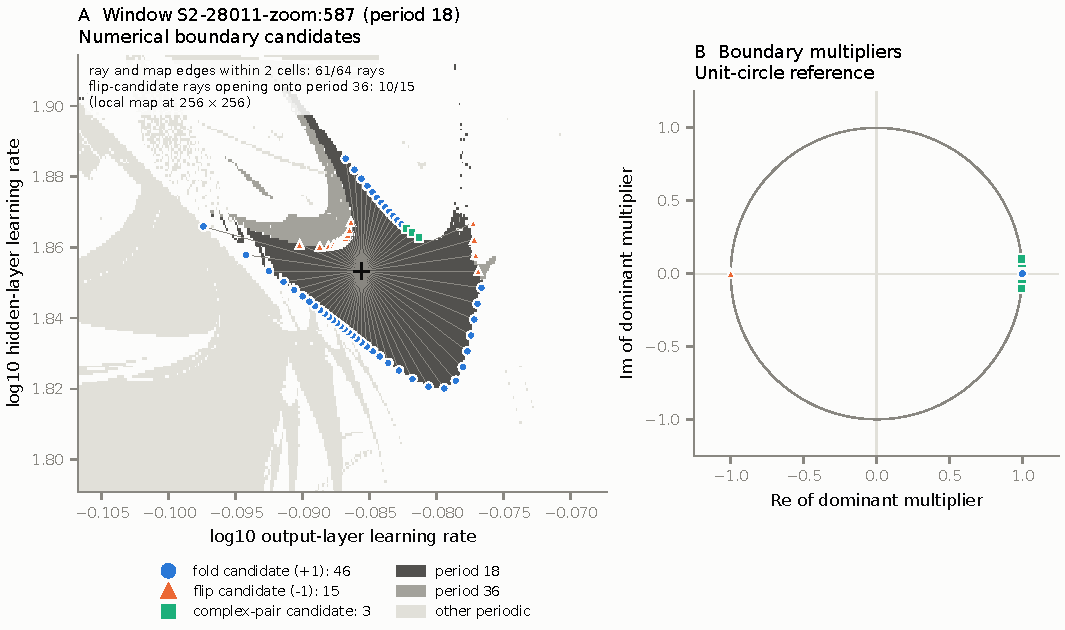
\includegraphics[width=\linewidth]{f4_window_anatomy.pdf}
\caption{\textbf{The period-18 window of S2-28011 has a fold-bounded body with flip edges opening onto
period-36 bands.} A: local map from the shared initial parameters with the window's orbit continued along 64
rays; markers show where and how it loses stability. B: crossing multipliers on the unit circle. This window was
selected as the clearest example and is one of only \nDraftShrimp{} meeting the draft shrimp criteria; it is not
representative (Figure~\ref{fig:census}).
\provenance{paper/gd-route/figures/f4\_window\_anatomy.py}{figures/f4\_window\_anatomy.provenance.json}}
\label{fig:anatomy}
\end{figure}

Draft criteria for classical shrimp anatomy require fold and flip boundaries each on at least 8 of 64 rays, at
least half of the flip rays opening onto period $2p$ in a local map, and agreement between ray and map edges on at
least three quarters of rays. \nWindowsFoldFlip{} windows meet the boundary-count part and \nDraftShrimp{} meet all
of it. The clearest, the period-18 window of S2-28011 (Figure~\ref{fig:anatomy}), has \nWFold{} fold, \nWFlip{}
flip and \nWNS{} complex-pair rays; ray and map edges agree within two cells on \nWEdgeAgree{} of \nWEdgeCompared{}
rays, and \nWFlipTwoP{} of its flip rays open onto period 36. Complex-pair boundaries, absent from classical
shrimps, are common: \nWindowsNS{} of \nConfirmed{} windows have at least 8 such rays.

\placeholder{Minimal model bridge: the two-mode depth-two linear network of \citet{hofmann2026} beyond its
rotational edge, testing whether the persistently misaligned oscillatory state is quasi-periodic, with a rotation
number continuous from the crossing angle, and whether it has locking windows (in progress).}

\placeholder{Prespecified route-to-chaos path: a connected path, fixed in advance, from the period-2 region
through the quasi-periodic band and locked windows into sustained chaos with converged diagnostics (not yet run).}

\placeholder{Bounded transfer to real data: a small network on a CIFAR subset, developed on a first subset with
everything frozen before a second subset is opened (not yet run).}

\placeholder{Consequences for training: the exploratory consequence pilot (reproducibility, stopping-time
sensitivity and loss against regime, with periodic and chaotic controls, and incremental value beyond the
Lyapunov exponent and sharpness), to be added with numbers generated from its receipts.}

\section{Discussion}
\label{sec:discussion}

Everything in this section is interpretation. The confirmed results in Section~\ref{sec:confirmed} stand on
their own, and the hypotheses here need their own prespecified tests.

The picture that fits the exploratory evidence is the quasi-periodic organization familiar from circle maps and
forced oscillators \citep{curry1978,aronson1982,jensen1984}: the edge-of-stability oscillation is a period-2
orbit; past a complex-pair crossing of the two-step map, training moves on an invariant circle with a rotation
number set by the crossing angle; rational rotations lock into periodic windows; and the circle breaks, with
period doubling inside locked windows along the way. Section~\ref{sec:background} explains why the crossing needs
at least period 2 in gradient descent and why per-layer rates are not required for it in principle; the rotational
edge of \citet{hofmann2026} is the same kind of crossing in a solvable model. Under this reading, most windows of
Section~\ref{sec:confirmed} are locked orbits, and classical shrimps are a special case.

\paragraph{Reading the rotation from the loss.} In exploratory analyses of the consequence pilot, the dominant peak
of the even-step training-loss spectrum tracked the two-step rotation number, and an autoregressive fit to noisy
loss recovered the period-2 orbit's complex multiplier before the crossing. We treat this as local system
identification, not early warning, until sampling, harmonic, abstention, autoregressive-baseline and specificity
rules are fixed in advance. The earliest spectral diagnostic of learning dynamics we know of is that of
\citet{vandermaas1990}, who used broadband spectra to recognize chaotic learning; here a spectral peak would carry
the rotation number.

\paragraph{Open questions.} The odd-period windows did not pass the Birkhoff diagnostic; whether they are organized
as in periodicity hubs \citep{jones2012} is open. Windows also coexist with other attractors, so maps started from
one initial point show which attractor that point reaches rather than the full existence region of a window. And
the evidence comes from two small networks.

\paragraph{The test that would settle the local claim.} An existence-and-replication test would fix in advance a
single primary endpoint (a bounded set of mechanism criteria: a simple transverse complex-pair crossing with all
other multipliers inside the circle, nondegeneracy, an attracting invariant circle with converged residuals,
rotation compared with the crossing angle at prespecified detunings, and ancestry of a rule-selected window through
both folds), and apply it to two prespecified independent losses across two architectures, one of them unused so
far, with no substitution.

\section{Limitations}
\label{sec:limits}

The networks have 13 and 72 parameters and are trained on synthetic data with deterministic full-batch updates
in float64. Screening labels are finite-time; chaotic labels rest on single-tangent exponents and reruns.
Certification is a floating-point verification. Rotation numbers and the Birkhoff test use two-dimensional
projections of curves that live in 13 or 72 dimensions. The mechanism analyses were chosen after seeing related
outcomes, and the staircase and crossing analyses cover two slices and one curve. No result addresses
generalization, training speed or modern training practice.

\section{Related work}
\label{sec:related}

\paragraph{Edge of stability.} \citet{cohen2021} describe the edge of stability; \citet{damian2023} explain
self-stabilization of sharpness at the edge, whereas we follow what happens after the period-2 oscillation itself
loses stability; \citet{agarwala2023} show progressive sharpening to the edge in second-order regression models,
the approach to the regime we study beyond it; \citet{lewkowycz2020} describe a catapult phase at large rates, in
which the loss first grows and then settles in flatter regions, while our maps resolve the long-run dynamics of
rates where training does not settle. Further analyses include \citet{kalra2025}, \citet{chenbruna2023},
\citet{song2023}, \citet{chen2024phases}, \citet{cohen2025central} and \citet{hofmann2026}.

\paragraph{Chaos and fractals in training.} Chaos in deterministic training is discussed by \citet{kong2020} and
\citet{jimenez2026}; fractal trainability boundaries by \citet{sohldickstein2024}, \citet{torkamandi2025},
\citet{liu2024} and \citet{liang2026}; riddled basins and reproducibility by \citet{ly2025}. Learning dynamics in
games show chaos \citep{sato2002} and phase locking \citep{metaxas2026}, for adaptive rules rather than descent on
one loss.

\paragraph{Dynamical systems.} Shrimp-shaped windows are described by \citet{gallas1993,gallas1994}; circle maps,
Arnold tongues, devil's staircases and the breakdown of invariant circles by
\citet{arnold1965,jensen1983,jensen1984,curry1978,aronson1982,ostlund1983}; numerical bifurcation analysis of maps
by \citet{kuznetsov2019}. A literature check using generic queries found no report of quasi-periodic training,
Arnold tongues or rotation-number staircases for optimizers acting on one loss.

\section{Reproducibility}
\label{sec:repro}

Code, plans and compact receipts live in the project repository; bulky raw maps live in a separate data store
referenced by SHA-256. Every figure is generated by a script in \path{paper/gd-route/figures/} that reads saved
evidence and writes a receipt with input hashes, the generator's hash, output hashes, alt text and the values it
displays. Every number in the text, and the design table, is generated by
\path{paper/gd-route/scripts/build_numbers.py}; \path{data/numbers.json} records each number's source file, hash
and computation, and \path{provenance.json} indexes all receipts. \path{paper/gd-route/scripts/verify.py}
regenerates every figure and number and fails on any difference. The verification status of every reference is
kept in \path{data/references-ledger.json}. The map study corresponds to the repository's EXP-028 plan and audit;
its plan, receipts and audit are linked from \path{docs/EXP-028-results.md}.

\placeholder{Author contributions, acknowledgments, license choice and public code and data links are human
decisions to be made before release.}

\bibliographystyle{plainnat}
\bibliography{references}

\end{document}
